\documentclass[conference]{IEEEtran}
\IEEEoverridecommandlockouts
% The preceding line is only needed to identify funding in the first footnote. If that is unneeded, please comment it out.
\usepackage{cite}
\usepackage{amsmath,amssymb,amsfonts}
\usepackage{algorithmic}
\usepackage{algorithm2e}
\usepackage{graphicx}
\usepackage{textcomp}
\usepackage{xcolor}
\usepackage{tikz}

\DeclareMathOperator*{\argmax}{argmax} % thin space, limits underneath in displays
\DeclareMathOperator*{\argmin}{argmin} % thin

\usepackage{rotating}
\usepackage{graphicx}
\usepackage{listings}
\usepackage{color}
\usepackage{cite}
\usepackage{multirow}
\usepackage{colortbl}
\usepackage{enumitem}

\usepackage[para]{threeparttable}
\usepackage{array,booktabs,longtable,tabularx,tabulary}
\newcolumntype{L}{>{\raggedright\arraybackslash}X}
\usepackage{ltablex}
\usepackage{siunitx}
%\usepackage{caption}%
\setlength{\LTcapwidth}{7in}
\usepackage[flushleft]{threeparttablex}

\usepackage{hyperref}

\def\BibTeX{{\rm B\kern-.05em{\sc i\kern-.025em b}\kern-.08em
    T\kern-.1667em\lower.7ex\hbox{E}\kern-.125emX}}
\begin{document}

\title{ECU Identification using
Step Response Characterization and Spectral Analysis with Neural Network Classification\\
{\footnotesize \textsuperscript{}}
}

\author{

\IEEEauthorblockN{Azeem Hafeez}
\IEEEauthorblockA{\textit{CECS Department} \\
\textit{University of Michigan}\\
Dearborn, USA \\
azeemh@umich.edu}
\and

\IEEEauthorblockN{Kunaal Verma}
\IEEEauthorblockA{\textit{CECS Department} \\
\textit{University of Michigan}\\
Dearborn, USA \\
vermakun@umich.edu}
}

% make the title area
\maketitle
% As a general rule, do not put math, special symbols or citations
\begin{abstract}
Controller area network (CAN) protocol has been the predominant in-vehicle network architecture used by automotive manufacturers over the past 30 years, and it has proven to be a reliable architecture for the scaling growth of vehicle electrical systems into the information age. As in-vehicle electrical architectures increase in complexity, so do their value as targets of cybersecurity attacks and intrusion. CAN, being a legacy architecture, does not have in-built capabilities that can handle these new threats to security and safety. Interest in developing security measures to bring cybersecurity capabilities to CAN shall increase as manufacturers get more pressure from internal program teams, customers, and regulators to offer cybersecurity protection on these systems, especially in the face of new technologies like vehicle sensor networks, autonomous control, and mobile connectivity. This may force some manufacturers to plan for adoptation of new in-vehicle network protocols earlier than planned, and potentially abandon institutional knowledge and prior development work using CAN.

This pressure can be alleviated by creating new methods of cybersecurity that can be applied to current CAN architectures. One such method, proposed by Hafeez et. al. \cite{hafeez2019}, shows a promising way of fingerprinting network messages with a combination of ECU/CAN Channel characteristization and Machine Learning algorithms.

In this work we investigate further improvements on this method, increasing the featurespace available for training of a neural network model to classify eight unique ECU/CAN Channel pairs. Added features are taken from the field of Spectral Anaylsis. In addition, a featurespace reduction is performed to optimize performance. With these additions and modifications, detection accuracy of this method increases to 98.76\%, while reducing the computational cost on the system.
\medbreak
\end{abstract}

\begin{IEEEkeywords}
Intrusion detection system (IDS), electronic control unit (ECU), controller area network (CAN), machine learning (ML), artificial neural network (ANN), performance matrix (PM), heuristic algorithms (HA), automotive electronics (AE).
\end{IEEEkeywords}

\maketitle

\section{Introduction}

Automotive electrical systems consist of several physically isolated Electronic Control Units (ECUs) that control various elements of the vehicles. Network messages are broadcast on an open bus architecture, where messages reach every ECU on the network. This topology is benefitial for free flow and access of information across the network, where and ECU can extract all the information they need from other ECUs while maintaing a low harness wiring cost.

Unfortunately, this also means that intrusive actors with physical access to the vehicle can spoof ECU messages quite easily, and there are growing concerns that they can also accomplish this remotely through increasing mobile network connectivity of modern vehicles.

As described in Hafeez et. al. \cite{hafeez2019}, a method of CAN-channel signal characterization can be used to identify known ECUs on the network. In their paper, they adopted step-response signal characteristics to accomplish this task, but additional features from other areas of signal processing may provide additional accuracy.

Once known ECUs have been successfully identified and integrated into a detection model, the fingerprinting system can be begin to detect and isolate unknown ECU signatures, as seen in Fig \ref{fig:NetworkTopology}.

\begin{figure}[htb]
\centering
\includegraphics[width=3.2in]{figures/01_Fingerprinting.png}
\caption{$CAN  \; Topology  \; with  \; ECU \;  Fingerprinting$}
\label{fig:NetworkTopology}
\end{figure}

The primary purpose of the system described in this paper is to verify messages coming from known ECUs using fingerprinting and pattern recognition techniques. It accomplishes this by relying on manufacturing and material variation in physical CAN channel wiring (material, length, shielding) and chipset/component part variance. An intrusive ECU can then be isolated using a fingerprinting module that runs in parallel with the network, sampling and checking messages to ensure unrecognized signals can be identified, alerted to, mitigated, ignored, and isolated.

\section{Dataset Preparation}

The dataset used in this paper is the same dataset used in Hafeez et. al. \cite{hafeez2019}, which includes CAN-High protocol data from 8 ECUs. Each ECU is recorded 30 times, with roughly 600 samples per record at 20 kHz. The records provided show a regular clock pulse from CAN-Hi Dominant Bit to Recessive Bit, with an 86\% duty-cycle of the Dominant Bit. CAN-Hi has two logic voltage levels: 3.5V for the Dominant Bit, 2.5V for the Recessive Bit. We will use this specification later when we calculate Steady-State Value (\ref{sec:SSV}), Steady-State Error (\ref{sec:SSE}), and Signal-to-Noise Ratio (\ref{sec:SNR}).

\begin{figure}[htb]
\centering
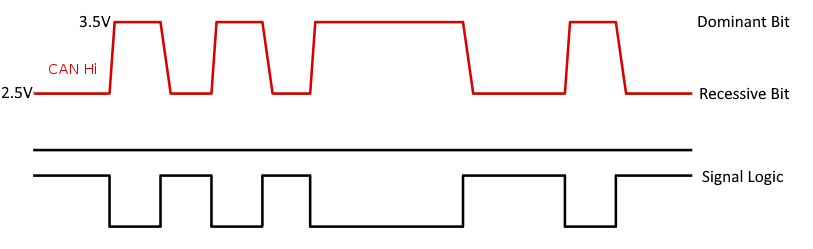
\includegraphics[width=3.2in]{figures/02_can_hi.png}
\caption{$CAN  \; Signal \; Logic  \; Voltage$}
\label{fig:CANBitLogic}
\end{figure}

Analyzing the CAN-Hi Signal using various fingerprinting methods will allow us to create ML classifiers of varying accuracy.

\section{Signal Processing Techniques}

A variety of tools are used to perform the signal processing necessary to detect and produce signal characteristics reliably. This section will review hot these processes operate and how they are used:

\subsection{Out-of-Bound Pulses}  \label{sec:OoBP}
There are sometimes instances in the dataset where a pulse cannot be cleanly extracted from the extreme ends of the raw data. In situations like this, the peak detection algorithm will errantly include indices for these pulses which could lead to skewing of signal characteristics.

To exclude these pulses, a logic function is used to measure the distance between similar bit pulses, and any pulse duration less than the average interval is removed. For a index vector $idx_{(n)}$ of size $n$, we check to see if any distance between peaks is less than the expected signal interval. For those indices that do not meet our desired criteria, we remove them from the peak index vector:
\medbreak
\begin{algorithmic}
\STATE $idx = [\;idx_{(0)} ... idx_{(n)}\;, idx_{(n)} + \textbf{interval\_length}\;]$
\medbreak
\STATE $idx[\;\textbf{DIFF}(idx) \leq \textbf{interval\_length}\;] = \textbf{EMPTY}$
\end{algorithmic}

\subsection{Convolution Filter}
The convolution filter (or moving average filter), uses a vector of ones of fixed length $w$ and convolves it with the interested vector in question. This creates and average of values within that window range for $n-w$ values in the target vector. In realtime, this creates a delay of $w$ samples, but in off-line processing we can prepend $w$ zeros to the start of the vector to account for the delay and maintain a vector of the same length as the original.
Depending on the window size chosen, this can sufficiently smooth noisy signal data without losing too much fundamental and lower harmonic energy. This becomes useful for various purposes including threshold, maxima, and minima detection. In other cases we choose larger window sizes of the filter in order to focus on lower frequency energy, as in the case of calculating Steady-State Value (\ref{sec:SSV}).
\medbreak
\begin{algorithmic}
\STATE $w = \textbf{window\_size} \text{ is odd}$
\STATE $v = [\;v_{(0)} ... v_{(n)},\;]$
\STATE $v_w = [ \textbf{ZEROS}((w-1)/2), \;v,\; \textbf{ZEROS}((w-1)/2)]$
\STATE $v_c = [\;]$
\FOR{$0 \le i \le \textbf{SIZE}(v)$}
    \STATE $v_c[i] = \textbf{SUM}(v_w[i:i+w])$
\ENDFOR
\end{algorithmic}

\subsection{Threshold Detection} \label{sec:Threshold}
Threshold detection is a relatively simple procedure that requires only a handful of steps. First, we subtract the threshold we are looking for from the vector of interest. Then, we perform an absolute value of the result. With this new signal, if we are able to isolate a subset of the vector that represents our region of  interest, we simply need to find the minimum value and its index:
\medbreak
\begin{algorithmic}
\STATE $val = [\;val_{(0)} ... val_{(n-1)}\;]$
\STATE $val\_t = val - \textbf{threshold}$
\STATE $val\_abs = \textbf{ABS}(val\_t)$
\STATE $val\_min = \textbf{MIN}(val\_abs) == val\_abs$
\STATE $val\_loc = \textbf{FIND}( val\_min ) $
\end{algorithmic}

\section{Feature Selection}

In the previous work by Hafeez et. al. \cite{hafeez2019} the featureset used for classification of specfic channels relied upon step response signal characteristics. The analysis performed in this paper will be repeat and confirm this work, and then go on to modify the featureset to include new features and remove features that prove to diminish performance unneccessarily.

Unique features added in this work use characteristics derived from the frequency spectrum content of the unique pulses. First, the Power Spectral Density of each pulse is processed, from which we can extract more specific values. The hope is to identify new characteristics that provide new and sufficiently varied values that will allow the machine learning procedure to better separate ECU messages and provide more accurate classification results.

\section{Step Response Acquisition}

The step response of Dominant and Recessive CAN-Hi bits are evaluated for a variety of characteristics is presented in the following section. The following steps walk through the signal processing requirements to extract these characteristics, their dependencies, and their limitations in providing valuable variation in the machine learning layer.

\subsection{Peak Detection (*)}
Peak Detection relies on using a smooth signal trace of the raw data signal in order to perform threshold comparisons reliably. For this reason, we employ a moving average filter to make the signal easier to manage:
\medbreak
\begin{algorithmic}
\STATE $w = \textbf{convolution\,window} = 6$
\STATE $t = \textbf{threshold\,window} = 0.2$
\STATE $val = [\;val_{(0)} ... val_{(n-1)}\;] $
\STATE $val\_dif = \textbf{DIFF}(\;val\;) $
\STATE $val\_mav = [\textbf{ZEROS}(w),\;\textbf{CONV}(\;val\_dif,\;w) $
\STATE $dom\_peaks = \textbf{FIND}(\;val\_mav > +t\;)$
\STATE $rec\_peaks = \textbf{FIND}(\;val\_mav < -t\;)$
\end{algorithmic}
\medbreak

After this stage, we analyze the indices to determine if there are errant peaks that are out of bound (\ref{sec:OoBP}). We also use some logic to ensure that the distance between Dominant and Recessive bits are also occuring as expected, and that we will be able to pair these peaks in order to extract full pulses correclty in processing other features (see Fig. \ref{fig:Peak}).

\begin{figure}[htb]
\centering
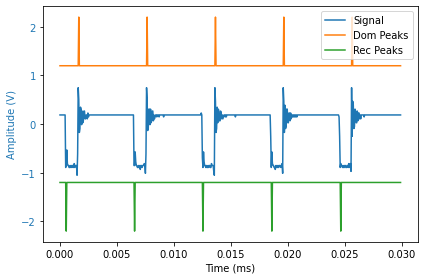
\includegraphics[width=3.2in]{figures/50_peak.png}
\caption{$Peak\;Detection\;Output$}
\label{fig:Peak}
\end{figure}

In practice, after removing DC bias from the signal, we found that $\pm 0.2$ V provided accurate peak index output.

\subsection{Pre-Peak Steady State Detection (*)}
\begin{figure}[htb]
\centering
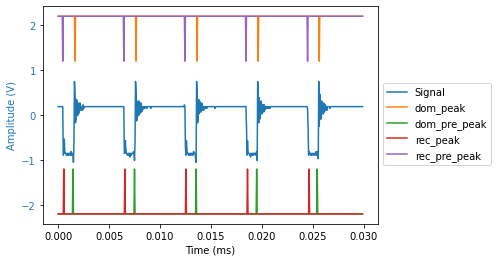
\includegraphics[width=3.2in]{figures/51_prepeak.png}
\caption{$Pre-Peak\;Detection\;Output$}
\label{fig:Prepeak}
\end{figure}

\subsection{Peak Time}
Peak Time is calculated by finding the difference between the start and end of the transient period. This can be done directly with a time series vector, or as in our case using index differences and scaling by the sampling period.
\begin{equation*}
T_p = (idx_{peak} - idx_{pre-peak}) * \textbf{sampling\,time}   
\end{equation*}

\subsection{Steady-State Value} \label{sec:SSV}
Steady-State Value requires a moving average filter window size approximately equal to the shorter bit pulse length, in this case the Recessive bit pulse duration of ~20 samples. In our code, we shortened this to a window of 19 samples as it seemed to provide more accurate results.
\medbreak
\begin{algorithmic}
\STATE $w = \textbf{convolution\,window} = 19$
\STATE $val = [\;val_{(0)} ... val_{(n-1)}\;] $
\STATE $val\_mav = [\;\textbf{ZEROS}(w),\;\textbf{CONV}(\;val,\;w)\;] $
\STATE $dom\_ssv = val\_mav[\;dom\_idx_{prepeak}\;]$
\STATE $rec\_ssv = val\_mav[\;rec\_idx_{prepeak}\;]$
\end{algorithmic}
\medbreak

\begin{figure}[htb]
\centering
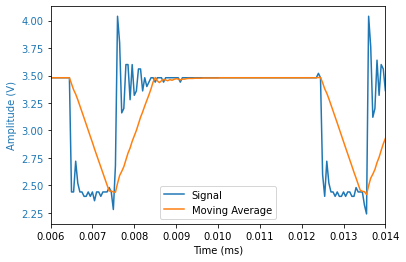
\includegraphics[width=3.2in]{figures/52_ssv.png}
\caption{$SSV\;Using\;Large\;Window\;Moving\;Average$}
\label{fig:SSV}
\end{figure}


\subsection{Steady-State Error} \label{sec:SSE}
Steady State Error relies upon knowledge of the CAN-Hi specificication, in which logical Dominant and Recessive values are stated as 3.5V and 2.5V, respectively. We take the $SSV$ and subtract with the respective logical bit voltage that we are looking for:
\begin{align*}
SSE &= SSV - V_{ideal,(bit)} \\ \text{ w} & \text{here } V_{ideal} =
    \begin{cases}
      3.5, & \text{if}\ bit=Dom \\
      2.5, & \text{if}\ bit=Rec 
    \end{cases}
\end{align*}

\subsection{Percent Overshoot}
Percent Overshoot measures the amount of overshoot that the rising edge of a pulse exceeds $SSV$:

\begin{equation*}
    \%OS = 100\% \times \frac{\text{Peak Amplitude} - SSV}{SSV}
\end{equation*}

\subsection{Settling Time}
Settling time takes several steps to compute. First, depending on the pulse under investigation, the $SSV$ is subtracted to debias the pulse signal. Second, an $\textbf{ABS}$ function is applied. Third, we use a moving average filter to create a signal envelope with which we can use a thresholding function to find the index at which the signal crosses 5\% of the $SSV$. In some cases, the signal will also need to be scaled in order to attain a logical 1 V$_{peak-to-peak}$. Luckily,due to the nature of Dominant and Recessive peak-to-peak voltage, we already accomplish this requirement.

\medbreak
\begin{algorithmic}
\STATE $w = \textbf{convolution\,window} = 3$
\STATE $val = [\;val_{(0)} ... val_{(n-1)}\;]$
\STATE $val\_abs = \textbf{ABS}(val - SSV)$
\STATE $val\_mav = [\;\textbf{ZEROS}(w),\;\textbf{CONV}(\;val\_abs,\;w)\;]$
\STATE $ $
\STATE $\text{Use Thresholding with } t = 0.05$
\end{algorithmic}
\medbreak

 Initial testing used a 2\% threshold, but the output values demonstrated some undesirable aliasing, so a greather threshold was chosen instead.

\begin{figure}[htb]
\centering
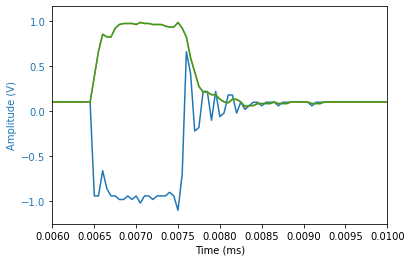
\includegraphics[width=3.2in]{figures/54_settling.png}
\caption{$Using\;Signal\;Envelope\;to\;find\;Settling\;Time$}
\label{fig:Settling}
\end{figure}

\subsection{Rise Time}
Rise Time is the amount of time the rising edge of a pulse reaches $SSV$. Determining this value requires using each pulses' calculated $SSV$ and the thresholding method discussed in Section \ref{sec:Threshold}.

\subsection{Delay Time}
Similar to Rise Time, Delay Time is the amount of time the rising edge of a pulse reaches $0.5\,SSV$. Determining this value requires using half of each pulses' calculated $SSV$ and the thresholding method discussed in Section \ref{sec:Threshold}.

\section{Spectral Analysis Acquisition}
Spectral Features of each pulse can be evaluated through the use of Fast Fourier Transform algorithms. It is understood that the reader has some familiarity with this class of algorithm as it is ubiquitously used in engineering theory. With a frequency spectrum representation of our signal to work with, we can also extract other unique features that can provide additional performance increases to our neural network model.

\subsection{Power Spectral Density}
The method for frequency spectrum transformation of pulse data used in this work utilizes Welch's method \cite{welch1967} to perform an efficient and fast Fourier transform of a sequential input vector (samples series data in our case). This algorithm is available as a simple function in \textit{scikitlearn} and produces a Power Spectral Density (PSD) data vector along with the associated frequencies based on a time series input and sampling frequency.

With PSD now available, we have to think about a way to include this information as a feature in our Machine Learning algorithm. While it is perfectly feasible to use the 200+ samples in the PSD vector, this can have an adverse effect on computation cost. Instead, we will choose to adopt frequency binning as a means of capturing spectral shape of the pulse frequency domain, but with a reduced number of values to ingest into our neural network training (Fig \ref{fig:PSDBin}).

\medbreak
\begin{algorithmic}
\STATE $> Isolate\;Pulses$
\STATE $>Perform\;FFT\;to\;produce\;PSD$
\STATE $nb = \textbf{number of bins}$
\STATE $bs = \textbf{bin size} = \textbf{ROUND}(\textbf{LEN}(PSD)/nb)$
\FOR{$0 \leq i \leq nb-1$}
    \STATE $idx\_start = i * bs$
    \STATE $idx\_end = (i+1) * bs$
    \IF{$idx\_end \geq \textbf{LEN}(PSD)$}
        \STATE $idx\_end = \textbf{LEN}(PSD) - 1$
    \ENDIF
    \STATE $PSD\_binned[i] = \textbf{AVG}( PSD[ idx\_start : idx\_end ] )$
\ENDFOR
\end{algorithmic}

\begin{figure}[htb]
\centering
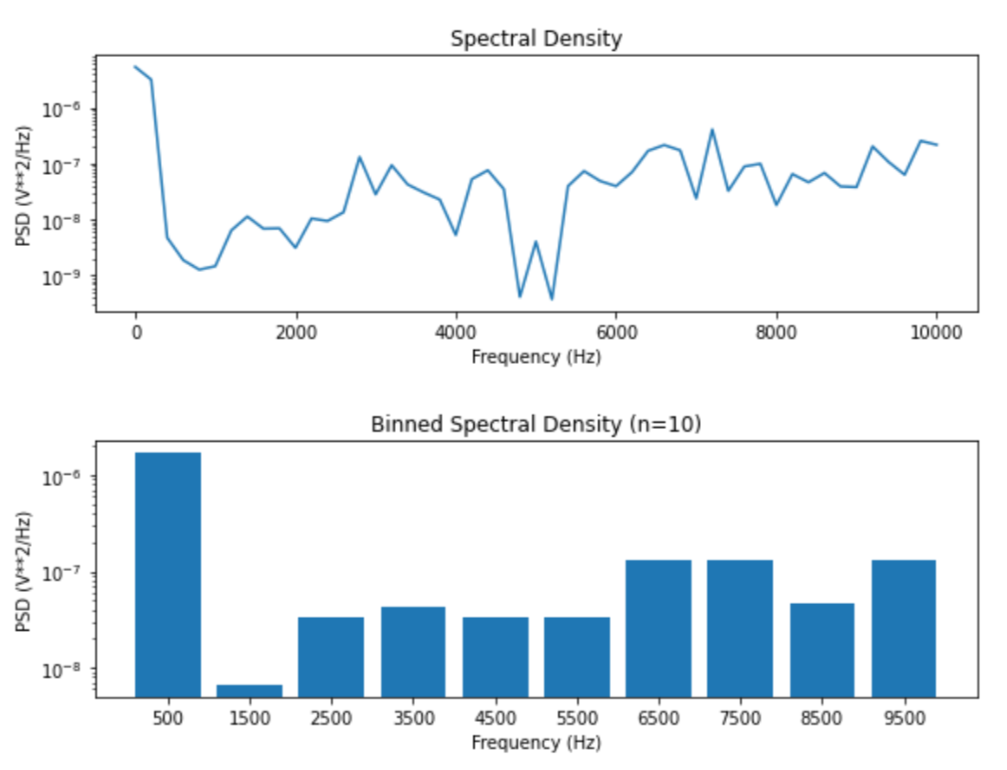
\includegraphics[width=3.2in]{figures/55_psd_bin.png}
\caption{$Bin-reduced\;Power\;Spectral\;Density$}
\label{fig:PSDBin}
\end{figure}

\subsection{Signal-to-Noise Ratio} \label{sec:SNR}
Signal-to-Noise Ratio measures the ratio between the power of the ideal pulse signal (a step function matched amplitude and peak synchronized to the raw signal) and the power of the signal noise (Fig. \ref{fig:SNR}).

\begin{align*}
    PSD&_{signal} = \textbf{FFT}(\textbf{Ideal Step Function})\\
    PSD&_{noise} = \textbf{FFT}(\text{Raw Signal Data} - \textbf{Ideal Step Function})\\
    SNR &= 10 \times log_{10} \frac{ \textbf{SUM}(PSD_{signal}) }{ \textbf{SUM}(PSD_{noise}) }
\end{align*}

\begin{figure}[htb]
\centering
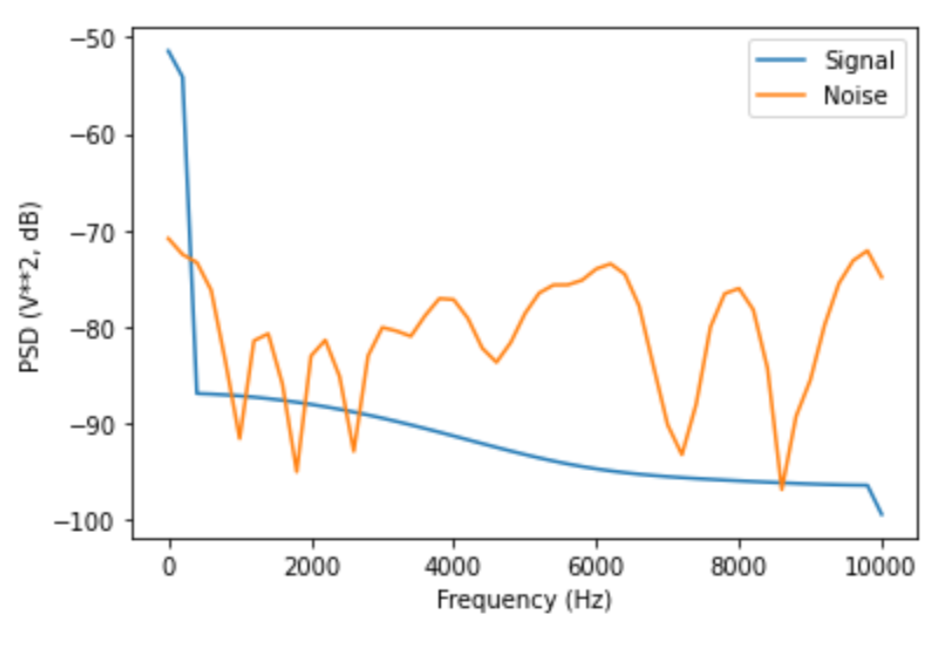
\includegraphics[width=3.2in]{figures/56_snr.png}
\caption{$Signal\;and\;Noise\;Power\;Spectral\;Density$}
\label{fig:SNR}
\end{figure}

\subsection{Mean Frequency}
Mean Frequency can be calculated directly from the PSD and frequency vector data produced by the FFT algorithm \cite{angkoon2012}:
\begin{equation*}
    MNF = \frac{ \sum_{j=1}^M f_j P_j }{ \sum_{j=1}^M P_j }
\end{equation*}

\subsection{Median Frequency}
Median Frequency is the frequency at which energy is split equivalent in the PSD \cite{angkoon2012}. PSD is normalized, cumulatively summed, offset by 0.5, and an absolute value is applied.  Median Frequency is found by locating the frequency at which a minima occurs in this data vector (Fig. \ref{fig:MDF}).

\begin{equation*}
    \sum_{j=1}^{MDF} P_j = \sum_{j=MDF}^(M) P_j = \frac{1}{2} \sum_{j=1}^{M} P_j
\end{equation*}

\medbreak
\begin{algorithmic}
\STATE $PSD,\;freq\_vec = \textbf{FFT}(\text{Raw\;Pulse\;Data})$
\STATE $PSD\_norm = PSD / \textbf{SUM}(PSD)$
\STATE $PSD\_cmsm = \textbf{CUMSUM}(PSD\_norm)$
\STATE $PSD\_off = PSD\_cmsm - 0.5$
\STATE $PSD\_abs = \textbf{ABS}(PSD\_off)$
\STATE $MDF = \textbf{FIND}( PSD\_abs == \textbf{MIN}(PSD\_abs) )$
\end{algorithmic}

\begin{figure}[htb]
\centering
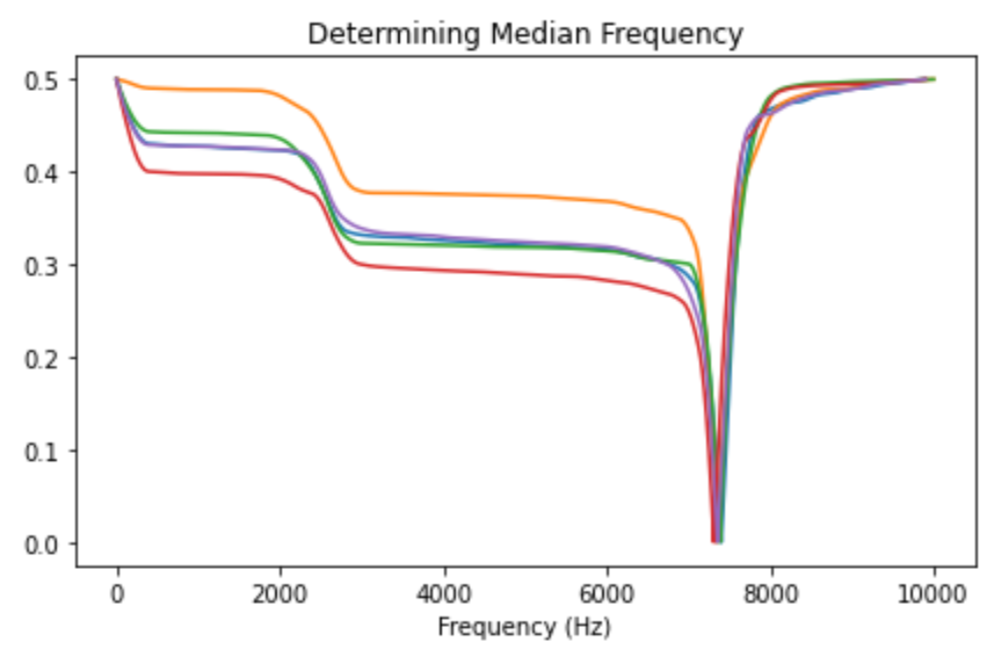
\includegraphics[width=3.2in]{figures/57_mdf.png}
\caption{$Median\;Frequency\;Calculation$}
\label{fig:MDF}
\end{figure}

\section{Feature Extraction}
A Python class was created to process all the above Acquisition functions for an input record file. The Record object was then parsed for the pertinent feature data, and copied to a Python data dictionary sequentially, in addition to file metadata that included $CAN\_Id$, $Channel\_Length$, $Channel\_Medium$, $ECU\_Record\_Id$, and $Filepath$.
Once this datadictionary was converted to a Pandas DataFrame, it could easily be parsed to produce the feature subsets to perform the machine learning process.

\section{Machine Learning Methodology}
Before training can occur, the dataset is split into a training and test set. A split of 70\% Training Data and 30\% Test Data was chosen. For the majority of development, this split in the data was not randomized in order to attain a consistent understanding of performance acrossing different subsets of features. After generalized performance was recorded, the training and datasets were completely randomized run to run in order to remove and training bias and overfitting that could influence performance results.

For all featuresets in this work, we trained a multi-layer perceptron neural network model to predict classifications for ECU in our testing set. We adopted use of the \textit{scikit-learn} MLPClassifier, which by default utilizes the Adam solver \cite{kingma2017adam}. For initial training, the hyperparameter values were chosen to be quite large in order to allow the solver to converge to a maximal solution. Early training typically used ~1000 Hidden Layers, ~3000 Epochs.

After the model was trained, the remaining testing records were used to measure performance of the model. A confusion matrix was constructed with the actual values of the test set, and the predicted values of the model.

\section{Performance Measurement}

To stay consistent with the previous work, we will be measuring performance using 5 metrics: accuracy, precision, recall, F1 score, and error. In order to accomplish this, we need to determine the True Position, True Negative, False Positive, and False Negative values for each class. These values can be easily extracted from a confusion matrix that compares the expected test values (actual) and the predicted test values output from our trained model.

\begin{figure}[htb]
\centering
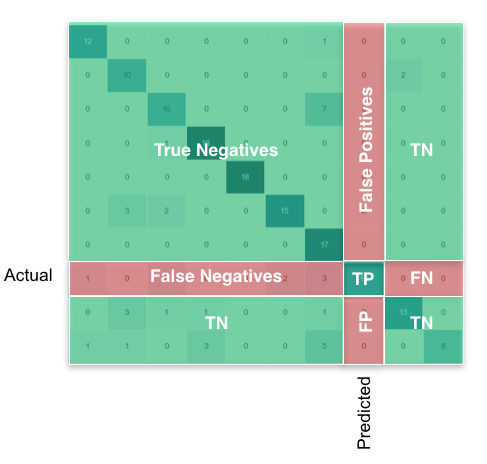
\includegraphics[width=3.2in]{figures/60_cm_pm.png}
\caption{$T/F  \; P/N \; Computation  \; from \; Confusion \; Matrix$ \cite{bell2020}}
\label{fig:CMPerfMetric}
\end{figure}

With these values, we can calculate our performance metrics for each class/ECU:

\begin{align*}
    Accuracy & = \frac{TP + TN}{TP + TN + FP + FN}\\\\
    Precision & = \frac{TP}{TP + FP}\\\\
    Recall & = \frac{TP}{TP + FN}\\\\
    F1\,Score & = 2 \times \frac{Precision \times Recall}{Precision + Recall}\\\\
    Error & = 1 - Accuracy
\end{align*}

\section{Feature Tuning}
Two Methods were evaluated initially using the Feature Extraction data:
\begin{enumerate}
    \item All Step Response Characteristics
    \item All Step Response + All Spectral Analysis Characteristics. 
\end{enumerate}
Figures \ref{fig:M1cm}-\ref{fig:M2pm} show the results of the featuresets. Overall, Method 2 showed less miss-classification between ECUs, with the biggest errors occuring with instances of CAN5 signals being mistaken for CAN1. Overall, Method 1 produced an average ECU classification accuracy of 96.85\%, and Method 2 produced accuracy of 98.28\%.

\begin{figure}[htb]
\centering
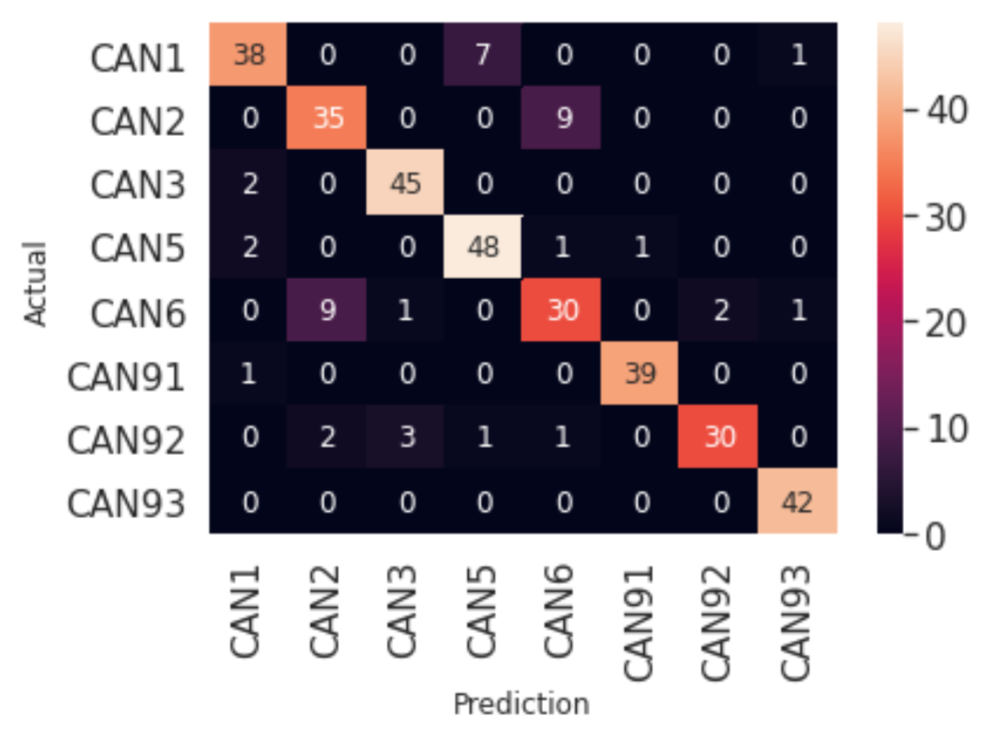
\includegraphics[width=3.2in]{figures/80_m1cm.png}
\caption{$Method\;1\;Confusion\;Matrix$}
\label{fig:M1cm}
\end{figure}

\begin{figure}[htb]
\centering
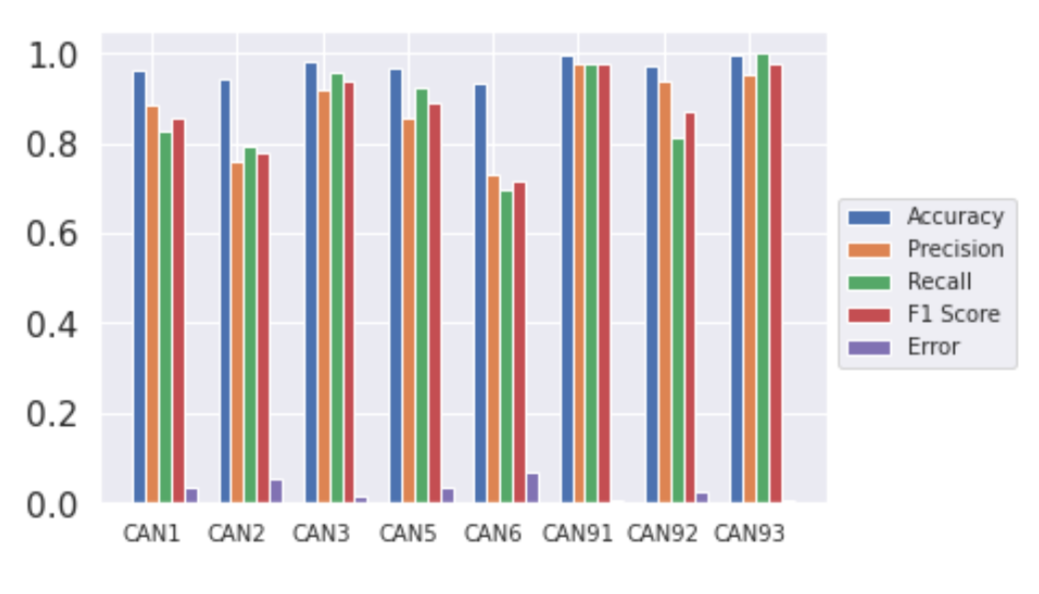
\includegraphics[width=3.2in]{figures/81_m1pm.png}
\caption{$Method\;1\;Performance\;Metrics$}
\label{fig:M1pm}
\end{figure}

\begin{figure}[htb]
\centering
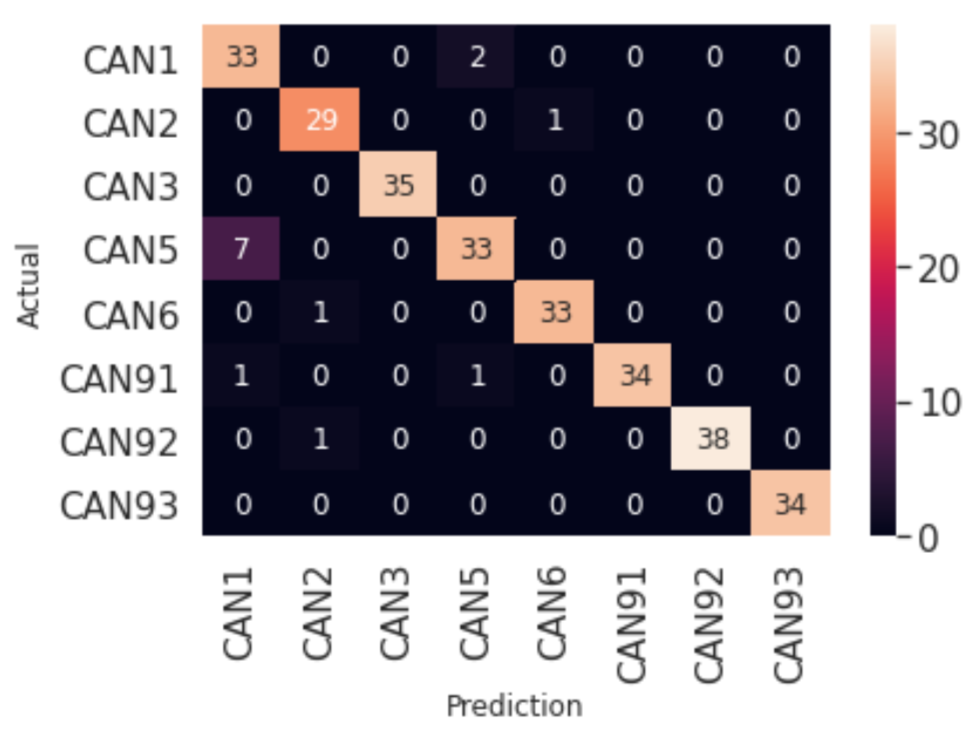
\includegraphics[width=3.2in]{figures/82_m2cm.png}
\caption{$Method\;1\;Confusion\;Matrix$}
\label{fig:M2cm}
\end{figure}

\begin{figure}[htb]
\centering
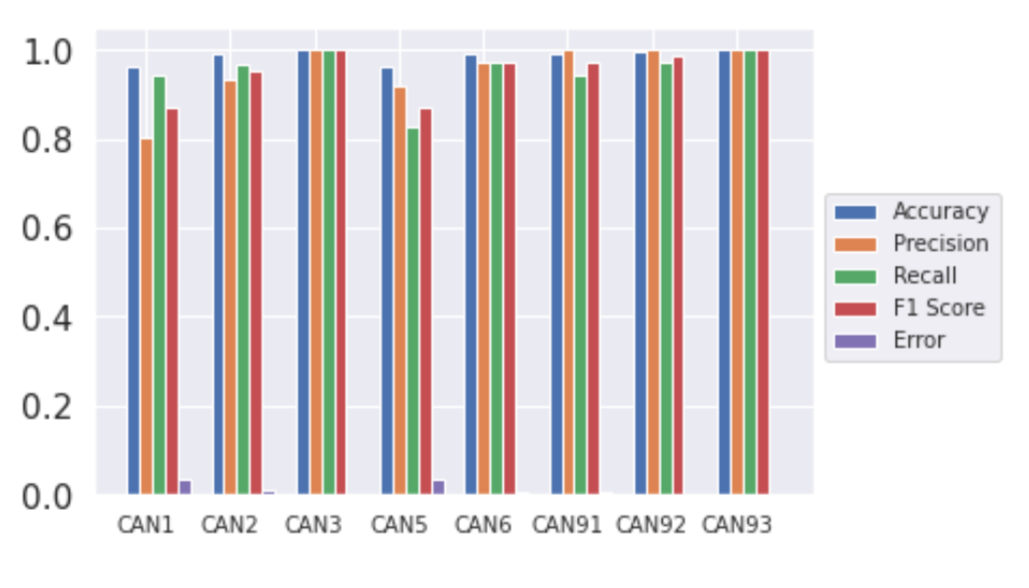
\includegraphics[width=3.2in]{figures/83_m2pm.png}
\caption{$Method\;2\;Performance\;Metrics$}
\label{fig:M2pm}
\end{figure}

With a baseline set, we looked to improve upon this accuracy by reducing the featureset. Since Method 2 proved to be more effective in its classification task (and it contained all features) we isolated each feature category and ran the neural network for each. With this output we ranked accuracy performance to identify the best performers in the featureset (Fig ).

\begin{figure}[htb]
\centering
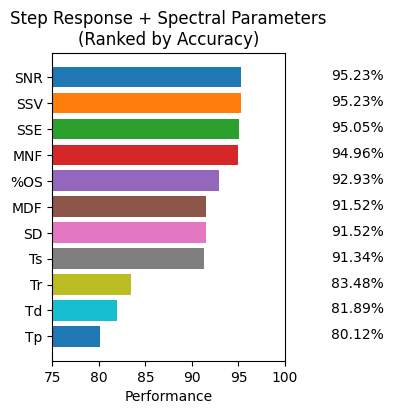
\includegraphics[width=3.2in]{figures/90_m2rank.png}
\caption{$Feature\;Accuracy\;Ranked$}
\label{fig:Rank}
\end{figure}

Next, we added features one by one and evaluated performance until we no longer saw an increase in overall accuracy.

\begin{figure}[htb]
\centering
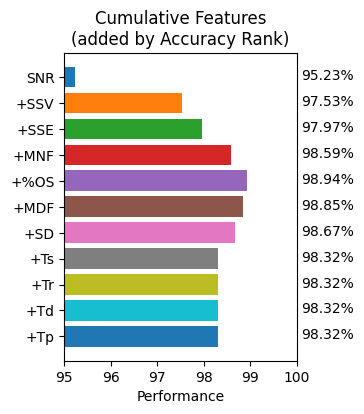
\includegraphics[width=3.2in]{figures/91_m2cumsum.png}
\caption{$Cumulative\;Feature\;Addition$}
\label{fig:CumRank}
\end{figure}

The final featureset included only $SNR$, $SSV$, $SSE$, $MNF$, and $\%OS$. Overall, we were able to exclude features that did not provide significant value to the overall peformane of the neural network model, reducing computational cost in the training of the model.

\section{Hyperparameter Tuning}

Although earlier testing picked relatively large values for neural network hyperparameters, with maximum epochs of 3000 and maximum hidden layers of 1000, we wanted to see if there were points of diminishing return for both hyperparameters. The full featureset was used in both test cases below. As we can see in Fig. \ref{fig:EpochPerf} Epoch performance converges at around 500. This bore out in practice during testing, and towards the end of analysis 500 epochs were used as the default value and adjusted accordingly to maximize accuracy performance for each featureset.

\begin{figure}[htb]
\centering
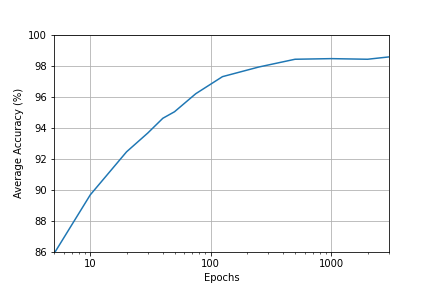
\includegraphics[width=3.2in]{figures/70_aa_vs_epoch.png}
\caption{$Average\,Accuracy\,Performance\,over\,Epoch\,Test\,Range$}
\label{fig:EpochPerf}
\end{figure}

As we can see in Fig. \ref{fig:LayerPerf}, Hidden Layer performance began to converge at around 1000 layers. In some situations, this convergence could be seen at around 100 layers given a sufficient number.

\begin{figure}[htb]
\centering
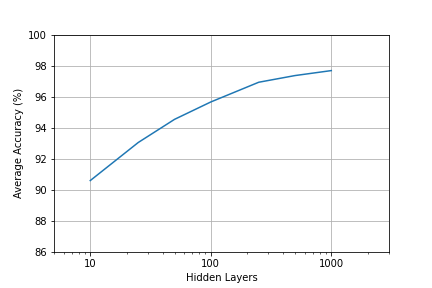
\includegraphics[width=3.2in]{figures/71_aa_vs_layers.png}
\caption{$Average\,Accuracy\,over\,Hidden\,Layer\,Test\,Range$}
\label{fig:LayerPerf}
\end{figure}

Finally, as we can see in  Fig. \ref{fig:TimePerf} we can see a sharp increase in performance as we increase from under 1 sec of compute time to 2 sec of compute time. After this period we see a moderate increase in performance as the solver continues to improve convergence. At around 8 sec of compute time we have reached our maximum performance, and any additional compute bears no more fruit. From the trial runs, this 8 sec run corresponds to situations in which the dataset was trained with 500 Hidden Layers and 500 Epochs. This is substantially less compute time than what we originally trained our network with, which could take up to 22 sec on our compute platform, Google Colab. This seems to be the sweetspot for this particular dataset and Training/Test set partition.

\begin{figure}[htb]
\centering
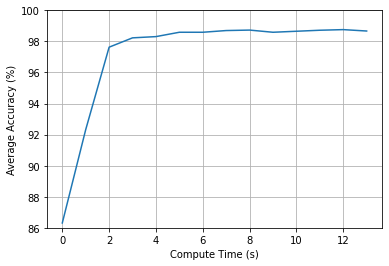
\includegraphics[width=3.2in]{figures/72_aa_vs_comp_time.png}
\caption{$Average\,Accuracy\,over\,Training\,Time$}
\label{fig:TimePerf}
\end{figure}

\section{Results}
With our final featureset, we ran 20 randomized trials using the MLP Classifier, with a hyperparameter optimzation of 275 Hidden Layers and 500 Epochs. This resulted in the performance metrics shown in Fig. \ref{fig:M2opt}. This model, with feature reduction and hyperparameter optimzation, led to an overall accurazy of 98.76\%.

\begin{figure}[htb]
\centering
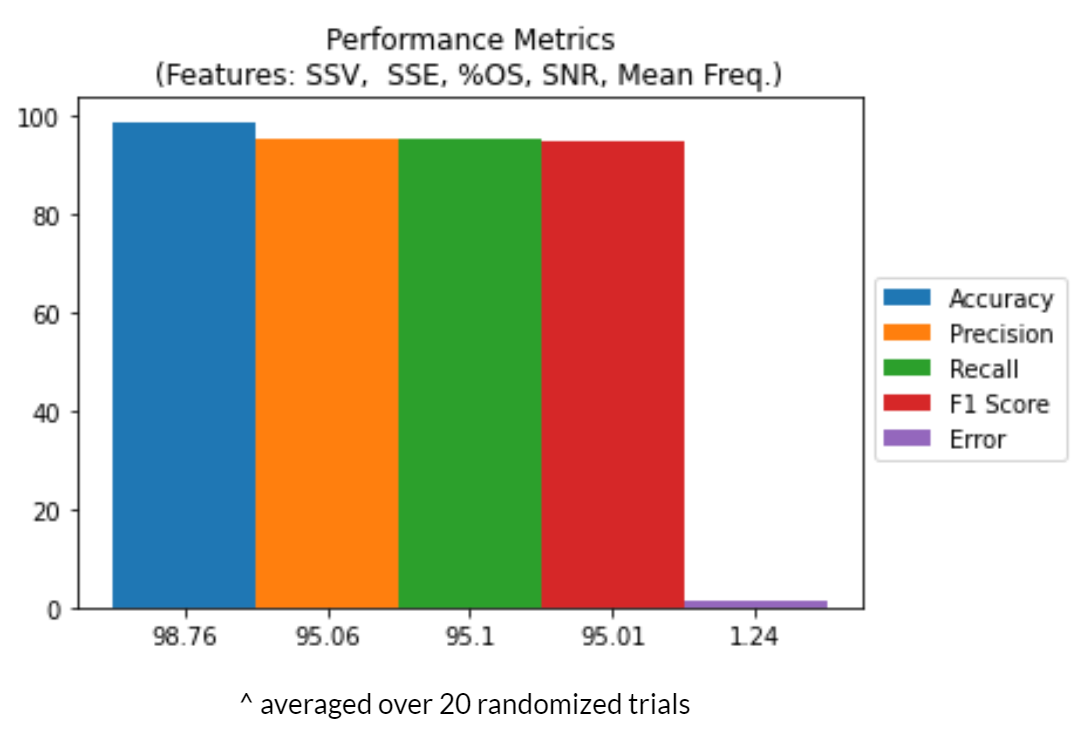
\includegraphics[width=3.2in]{figures/100_m2optperf.png}
\caption{$Optimal\;Method\;2\;Performance\;Metrics$}
\label{fig:M2opt}
\end{figure}

A similar optimization was performed on only the Method 1 featureset, resulting in slightly poorer performance as seen in Fig. \ref{fig:M1opt} with 97.17\% accuracy.

\begin{figure}[htb]
\centering
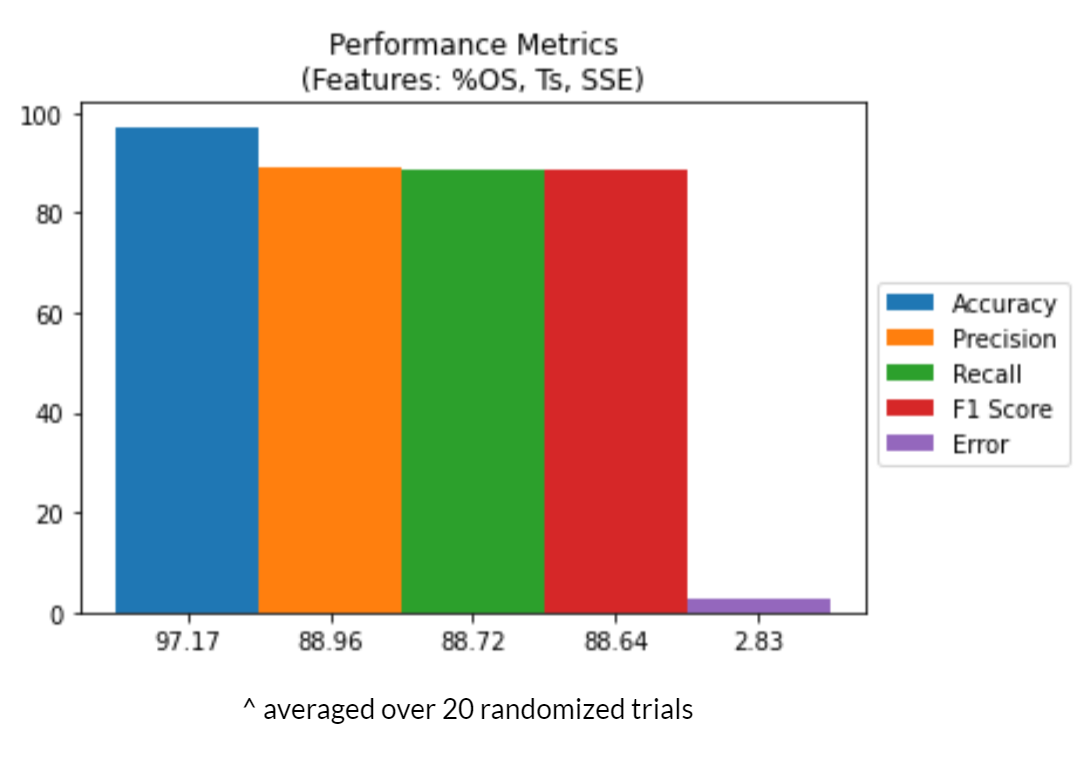
\includegraphics[width=3.2in]{figures/101_m1optperf.png}
\caption{$Optimal\;Method\;1\;Performance\;Metrics$}
\label{fig:M1opt}
\end{figure}

A comparison of all primary methods is shown in Fig. \ref{fig:final}. As we can see, the optimized Method 2 performed best, and had similar standard deviation to the other methods, save for the optimized Method 1.

\begin{figure}[htb]
\centering
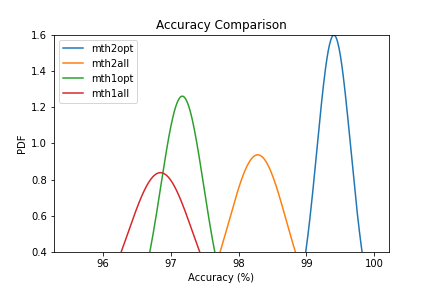
\includegraphics[width=3.2in]{figures/102_mth_comp.png}
\caption{$Comparison\;of\;Methods$}
\label{fig:final}
\end{figure}

\section{Conclusion}
\label{sec:concl}

This article expands upon existing work that establishes vehicle network ECUs and their associated physical channels can demonstrate significant channel-specific variance, so much so that signal-characteristics transmitted by each ECU can be uniquely identified. This can allow older vehicle network topologies that carry inherent cybersecurity weakness to mitigate intrusion by using a fingerprinting system to classify known ECUs on network, and identify rogue messages that may originate from local intrusion. The novelty of the methods in this paper add new features to the machine learning procedure and optimizes feature selection through a feature reduction pass. New features include signal-characteristics from the domain of Spectral Analysis, in particular Power Spectral Density, SNR, Mean Frequency, and Median Frequency. The feature reduction pass performs a quasi-heuristic search of feature combinations in order to maximize performance to computation ratio. Additionally, a similar quasi-heuristic search process is used to optimize hyperparameter values for the multi-layer perceptron neural network. All of these factors combined result in a channel detection accuracy of 98.76\%. Further investigation into dynamic online classification to account for channel degradation and changing global noise factors can be focused upon in future work. Another follow-up topic of interest is further reduction in network complexity of the MLPClassifier model and analyzing the performance of various sized models on commodity hardware. This would include

\newpage
\pagebreak

\bibliographystyle{IEEEtran}
% argument is your BibTeX string definitions and bibliography database(s)
%\bibliography{IEEEabrv,IEEEexample}
\bibliography{ece5831_project}

\end{document}